\documentclass[11pt, oneside]{article} 
\usepackage{geometry}
\geometry{letterpaper} 
\usepackage{graphicx}
	
\usepackage{amssymb}
\usepackage{amsmath}
\usepackage{parskip}
\usepackage{color}
\usepackage{hyperref}

\graphicspath{{/Users/telliott/Github/figures/}}
% \begin{center} \includegraphics [scale=0.4] {gauss3.png} \end{center}

\title{Basic number theory}
\date{}

\begin{document}
\maketitle
\Large

%[my-super-duper-separator]

Consider two natural numbers $a$ and $b$.  Usually $a$ is allowed to be an integer (i.e., it can be negative), but to keep things simple here we will say that $a,b \in \mathbb{N}$, $a$ and $b$ are positive integers.

We can find their \emph{greatest common divisor}, written $(a,b)$.  First we write the unique prime factorization of $a$ and $b$:

\begin{verbatim}
180 =          2 x 2 x 3 x 3 x 5
140 =          2 x 2 x         5 x 7
gcd(140,180) = 2 x 2 x         5 = 20
\end{verbatim}

Pick out the common factors and the gcd$(a,b)$ will be their product.  It is important that we do not need to actually factor $a$ and $b$.

(We will develop a theorem on unique prime factorization in another chapter).

The algorithm works like this.  Find integers $r \ge 0$ and $q > 0$ such that

\[ a = b \cdot q + r \]

$\bullet$ If $r = 0$ we are done:  $b$ divides $a$ equally.  Otherwise

$ \circ$ switch $a = b$ and $b = r$ and repeat.

Then $b$ is the gcd of the original $a$ and $b$.  

In our example

\begin{verbatim}
180 = 140 x 1 + 40
140 =  40 x 3 + 20
 40 =  20 x 2 + 0
gcd =  20
\end{verbatim}

Here is the reason this works.  First, we can always find $q$ and $r$ such that
\[ a = b \cdot q + r \]
This is a version of the Archimedean property for positive integers.  
\begin{center} 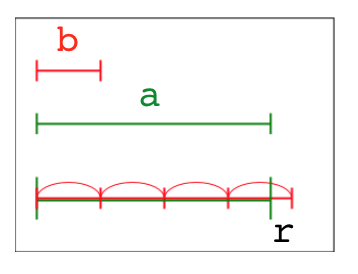
\includegraphics [scale=0.4] {Archimedean_property2.png} \end{center}
It may be paraphrased by saying
\begin{quote}given a bathtub full of water and a teaspoon, it is possible to empty the bathtub.\end{quote}


Either $a = b \cdot q$ and we are done or:
\[ b \cdot q < a < b \cdot q + b \]
So then
\[ a - bq > 0 \]
\[ a - bq < b \]
With  $r = a - bq$, we obtain $0 < r < b$.

Let $u$ be the largest integer that divides both $a$ and $b$ (the greatest common divisor)
\[ a = su \]
\[ b = tu \]
Then 
\[ su = q \cdot tu + r \]
\[ r = su - q \cdot tu \]
\[ r = u(s - q \cdot t) \]
So $u$ divides $r$.

Hence every common divisor of $a$ and $b$ is also a divisor of $b$ and $r$.

\subsection*{recursive program}

Here are two examples of programs in different styles that implement the algorithm (with no error checking):

\begin{verbatim}
def gcd(a,b):
    r = a % b
    if r == 0:
        return b
    return gcd(b,r)
\end{verbatim}

\begin{verbatim}
def gcd(a,b):
    r = a % b
    while r != 0:
        a,b = b,r
        r = a % b
    return b
\end{verbatim}

The first version is \emph{recursive}, it may call itself.  The second uses a \textbf{while} loop to accomplish the same thing.

\end{document}